\begin{enumerate}[label=\thesection.\arabic*.,ref=\thesection.\theenumi]
\numberwithin{equation}{enumi}
\item The transfer function of causal L.T.I system is 
\begin{align}
H(s) = \frac{1}{s}. 
\end{align}If the input to the system is 
\begin{align}
x(t) = (\frac{sin(t)}{\pi t})u(t)
\end{align}
, where u(t) is a unit step function, the system output 
$y(t)$ as $t \to \infty$  is ?

\solution
let
\begin{align}
    f(t) = sin(t)u(t)
\end{align}
We know that, 
\begin{align}
\mathcal{L}{f(t)} = F(s) = \frac{1}{1 + s^2} 
\end{align}
    (by u.v rule of integration.)

By using,  

\begin{align}
  \mathcal{L}{\frac{f(t)}{t}} = \int_{s}^{\infty}F(s) \dd{s} 
\end{align}

\begin{align}
\implies X(s) = (1/ \pi)( \frac{\pi}{2} - \tan^{-1}(s))
\end{align}
\begin{align}
\implies Y(s) = (1/ \pi s) ( \frac{\pi}{2} - \tan^{-1}(s)) 
\end{align}
since 
\begin{align}
Y(s) = X(s)H(s)
\end{align}
Then using Final Value theorem,
\begin{align}
y(\infty) = \lim_{s\to 0} sY(s) =(\frac{1}{\pi}) ( \frac{\pi}{2} - \tan^{-1}) = \frac{1}{2}
\end{align}





\textbf{ Proof of Final Value Theorem:}

To prove : 
\begin{align}
 \lim_{s\to\ 0} (sF(s)) = \lim_{t\to\infty} f(t)
\end{align}
We know,
\begin{align}
\mathcal{L}\{\pdv{f(t)}{t}\} = \int_{0^-}^{\infty} \pdv{f(t)}{t} e^{-st}\dd{t} =s*F(s)-f(0^{-})
\end{align}

Now applying $ s \to 0$
We have,
\begin{align}
 RHS =\int_{0^-}^{\infty} \pdv{f}{t}\dd{t} = \lim_{s\to\ 0}(f(\infty) - f(0^{-})) 
\end{align}
And
\begin{align}
    LHS= \lim_{s\to\ 0}(sF(s)-f(0^{-}))
\end{align}
Hence proved
\newline
\newline
\textbf{Plotting y(t) in time domain.}
\begin{lstlisting}
https://github.com/Kkuntal990/Control-theory-course/blob/master/codes/EE18BTECH11028.py
\end{lstlisting}
\begin{figure}[!h]
  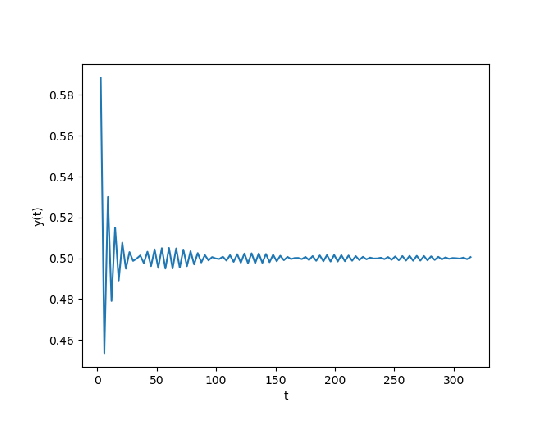
\includegraphics[width=\columnwidth]{EE18BTECH11028.eps}
\end{figure}

This shows as $t$ goes to infinity $y(t)$ tends to 0.5.
\end{enumerate}
